\documentclass[aspectratio=169,11pt]{beamer}

\usepackage[utf8]{inputenc}
\usepackage[T1]{fontenc}
\usepackage{lmodern}
\usepackage{amsmath,amssymb,mathtools}
\usepackage{booktabs}
\usepackage{xcolor}
\usepackage{graphicx}

\usetheme{Madrid}
\definecolor{BootcampBlue}{RGB}{31,78,121}
\definecolor{BootcampGold}{RGB}{215,155,35}
\definecolor{BootcampRed}{RGB}{176,48,48}
\definecolor{BootcampGreen}{RGB}{42,120,83}
\setbeamercolor{structure}{fg=BootcampBlue}
\setbeamercolor{alerted text}{fg=BootcampRed}
\setbeamercolor{example text}{fg=BootcampGreen}
\setbeamercolor{block title}{bg=BootcampBlue,fg=white}
\setbeamercolor{block body}{bg=BootcampBlue!5}
\setbeamercolor{title}{fg=white}
\setbeamertemplate{navigation symbols}{}

\newenvironment{resultblock}[1]{%
  \setbeamercolor{block title}{fg=black,bg=BootcampGold}%
  \setbeamercolor{block body}{fg=black,bg=BootcampGold!10}%
  \begin{block}{#1}}{\end{block}}

\newcommand{\R}{\mathbb{R}}
\newcommand{\E}{\mathbb{E}}
\newcommand{\trans}{^{\mathsf T}}
\newcommand{\grad}{\nabla}
\newcommand{\argmin}{\operatorname*{arg\,min}}
\newcommand{\proj}{\operatorname{proj}}
\newcommand{\prox}{\operatorname{prox}}

\title{Summer Bootcamp\\Session 3 -- Optimization}
\subtitle{Optimality, convexity, algorithms, constraints, and finance}
\author{Nathan Sauldubois}
\institute{NYU Finance and Risk Engineering}
\date{August 2026}

\AtBeginSection[]{
  \begin{frame}[plain]
    \sectionpage
  \end{frame}
}

\begin{document}

\begin{frame}
  \titlepage
\end{frame}

\begin{frame}{Roadmap}
  \tableofcontents
\end{frame}

% -----------------------------------------------------------------------------
\section{Formulating an optimization problem}

\begin{frame}{The common language}
  A generic optimization problem is
  \[
    \min_{x\in\R^d} f(x)
    \quad\text{subject to}\quad
    h(x)=0,\qquad g(x)\leq 0.
  \]

  \begin{itemize}
    \item $x$: decision variable;
    \item $f$: objective function;
    \item $\mathcal F=\{x:h(x)=0,\ g(x)\leq0\}$: feasible set;
    \item $x^\star$: optimizer, if $f(x^\star)\leq f(x)$ for every feasible $x$.
  \end{itemize}

  Maximizing $f(x)$ is the same as minimizing $-f(x)$.
\end{frame}

\begin{frame}{Three recurring financial problems}
  \begin{block}{Calibration / regression}
    \[
      \min_\theta \frac12\|A\theta-b\|_2^2.
    \]
    Calibration means choosing model parameters $\theta$ so that model outputs
    are as close as possible to observed market or historical data.
  \end{block}

  \begin{block}{Minimum-variance portfolio}
    \[
      \min_w \frac12 w\trans\Sigma w
      \quad\text{s.t.}\quad \mathbf 1\trans w=1.
    \]
  \end{block}

  \begin{block}{Constrained allocation}
    \[
      \min_w \frac12 w\trans\Sigma w-\gamma\mu\trans w
      \quad\text{s.t.}\quad \mathbf 1\trans w=1,\quad w\geq0.
    \]
  \end{block}
\end{frame}

\begin{frame}{Worked Example: Translate Words into Mathematics}
  A trader fits a linear model $y_i\approx a+bt_i$ and wants the smallest squared error.

  \medskip
  \textbf{Task.} Identify the decision variable, the objective, and the constraints.

  \pause
  \[
    x=\begin{pmatrix}a\\b\end{pmatrix},
    \qquad
    \min_{a,b}\frac12\sum_{i=1}^n(a+bt_i-y_i)^2.
  \]
  There is no constraint: $\mathcal F=\R^2$.

  \pause
  In matrix form, with $A_i=(1,t_i)$ and $y=(y_i)$,
  \[
    \min_x \frac12\|Ax-y\|_2^2.
  \]
\end{frame}

\begin{frame}{Your Turn: Formulate a Constrained Tracking Problem}
  A manager chooses weights $w\in\R^d$ so that portfolio returns
  $w\trans r_t$ track benchmark returns $b_t$, where $b_t$ is the return at
  date $t$ of a reference index or strategy used to evaluate the portfolio.
  The portfolio must be fully invested and long-only.

  \begin{exampleblock}{Task}
    Identify the decision variable, objective, and feasible set.
  \end{exampleblock}

  \pause
  With $R$ containing the asset returns and $b$ the benchmark returns,
  \[
    \boxed{
    \min_{w\in\R^d}\frac12\|Rw-b\|_2^2
    \quad\text{s.t.}\quad \mathbf1\trans w=1,\quad w\geq0.}
  \]
  The decision variable is $w$ and the feasible set is the long-only simplex.
\end{frame}

\begin{frame}{Local versus global minimum}
  \begin{itemize}
    \item $x^\star$ is a \textbf{local minimum} if it wins against nearby feasible points.
    \item $x^\star$ is a \textbf{global minimum} if it wins against all feasible points.
  \end{itemize}

  \begin{alertblock}{The central difficulty}
    Derivatives provide local information. Optimization usually asks for a global answer.
  \end{alertblock}

  Convexity will be the bridge between the two.
\end{frame}

% -----------------------------------------------------------------------------
\section{Unconstrained optimality}

\begin{frame}{First-order necessary condition}
  \begin{resultblock}{Result -- First-order criticality condition}
  Let $f:\R^d\to\R$ be differentiable and let $x^\star$ be an interior local minimum.
  Then
  \[
    \boxed{\grad f(x^\star)=0.}
  \]
  \end{resultblock}

  Indeed, for every direction $v$,
  \[
    \phi(t)=f(x^\star+tv)
  \]
  has a local minimum at $t=0$, hence
  \[
    0=\phi'(0)=\grad f(x^\star)\trans v.
  \]
  This holds for every $v$, so the gradient must vanish.

  \begin{alertblock}{Warning}
    A stationary point need not be a minimum.
  \end{alertblock}
\end{frame}

\begin{frame}{Second-order information}
  \begin{resultblock}{Result -- Second-order classification}
  Around a stationary point $x^\star$,
  \[
    f(x^\star+h)
    =f(x^\star)+\frac12h\trans\grad^2f(x^\star)h+o(\|h\|^2).
  \]

  Hence:
  \begin{itemize}
    \item $\grad^2f(x^\star)\succ0$ $\Rightarrow$ strict local minimum;
    \item $\grad^2f(x^\star)\prec0$ $\Rightarrow$ strict local maximum;
    \item the Hessian is indefinite $\Rightarrow$ saddle point;
    \item a semidefinite Hessian may be inconclusive.
  \end{itemize}
  \end{resultblock}
\end{frame}

\begin{frame}{Reminder: Positivity of a Symmetric Matrix}
  Let $H=H\trans$. Its quadratic form is $q_H(z)=z\trans Hz$.

  \begin{resultblock}{Definitions}
  \[
  \begin{aligned}
  H\succ0
    &\Longleftrightarrow z\trans Hz>0 &&\text{for every }z\neq0,
    &\text{positive definite},\\
  H\succeq0
    &\Longleftrightarrow z\trans Hz\geq0 &&\text{for every }z,
    &\text{positive semidefinite},\\
  H\prec0
    &\Longleftrightarrow z\trans Hz<0 &&\text{for every }z\neq0,
    &\text{negative definite}.
  \end{aligned}
  \]
  \end{resultblock}

  If $z\trans Hz$ takes both positive and negative values, $H$ is
  \textbf{indefinite}.
\end{frame}

\begin{frame}{Easy Characterizations of Matrix Positivity}
  \begin{resultblock}{Eigenvalue test in any dimension}
  For symmetric $H$:
  \[
  H\succ0\iff\lambda_i(H)>0\ \forall i,
  \qquad
  H\succeq0\iff\lambda_i(H)\geq0\ \forall i.
  \]
  Eigenvalues of both signs mean that $H$ is indefinite.
  \end{resultblock}

  \pause
  For $H=\begin{pmatrix}a&b\\b&c\end{pmatrix}$, determinant tests are immediate:
  \[
  \boxed{
  \begin{array}{rcl}
  H\succ0&\Longleftrightarrow&a>0\text{ and }ac-b^2>0,\\
  H\prec0&\Longleftrightarrow&a<0\text{ and }ac-b^2>0,\\
  H\text{ indefinite}&\Longleftrightarrow&ac-b^2<0.
  \end{array}}
  \]
  More generally, Sylvester's criterion uses the leading principal minors.
\end{frame}

\begin{frame}{Example: Stationary Points in One Dimension}
  Consider
  \[
    f(x)=x^3-3x^2+2.
  \]
  \textbf{Task.} Find and classify all stationary points.

  \pause
  \[
    f'(x)=3x(x-2),
  \]
  so the candidates are $x=0$ and $x=2$.

  \pause
  Since $f''(x)=6x-6$,
  \[
    f''(0)=-6<0 \Rightarrow \text{local maximum},
    \qquad
    f''(2)=6>0 \Rightarrow \text{local minimum}.
  \]
\end{frame}

\begin{frame}{Example: A Two-Dimensional Quadratic}
  Let
  \[
    f(x,y)=x^2+xy+y^2-4x-2y.
  \]
  The first-order condition gives
  \[
    \grad f(x,y)=
    \begin{pmatrix}2x+y-4\\x+2y-2\end{pmatrix}=0,
    \qquad (x^\star,y^\star)=(2,0).
  \]

  \pause
  Moreover,
  \[
    H_f=\begin{pmatrix}2&1\\1&2\end{pmatrix},
    \qquad
    2>0,\quad \det(H_f)=3>0.
  \]
  Hence $H_f\succ0$: $(2,0)$ is the unique strict global minimum.
\end{frame}

\begin{frame}{Example: Why Stationarity Is Not Enough}
  Consider $f(x,y)=x^2-y^2$. We have $\grad f(0,0)=0$, but
  \[
    H_f=\begin{pmatrix}2&0\\0&-2\end{pmatrix},
    \qquad \det(H_f)=-4<0.
  \]
  Thus $H_f$ is indefinite.

  \pause
  Equivalently,
  \[
    f(t,0)=t^2>0,
    \qquad
    f(0,t)=-t^2<0
  \]
  for $t\neq0$. The function increases in one direction and decreases in
  another: $(0,0)$ is a \textbf{saddle point}.
\end{frame}

\begin{frame}{Worked Example: Classify with the Hessian}
  Classify the origin for
  \[
    f_1(x,y)=x^2+4xy+5y^2,
    \qquad
    f_2(x,y)=x^2-4xy+y^2.
  \]

  \pause
  \[
    H_1=\begin{pmatrix}2&4\\4&10\end{pmatrix},
    \qquad
    \det H_1=20-16=4>0,\quad (H_1)_{11}>0.
  \]
  Thus $H_1\succ0$: the origin is a strict minimum.

  \pause
  \[
    H_2=\begin{pmatrix}2&-4\\-4&2\end{pmatrix},
    \qquad
    \det H_2=4-16=-12<0.
  \]
  Thus $H_2$ is indefinite: the origin is a saddle point.
\end{frame}

\begin{frame}{Your Turn: Classify Two Quadratic Forms}
  Classify the origin for
  \[
    g_1(x,y)=3x^2+2xy+2y^2,
    \qquad
    g_2(x,y)=-x^2-xy-y^2.
  \]

  \begin{exampleblock}{Task}
    Compute both Hessians and use the $2\times2$ determinant test.
  \end{exampleblock}

  \pause
  \[
    H_{g_1}=\begin{pmatrix}6&2\\2&4\end{pmatrix},
    \quad 6>0,\quad \det(H_{g_1})=20>0,
  \]
  so the origin is a strict minimum of $g_1$. Moreover,
  \[
    H_{g_2}=\begin{pmatrix}-2&-1\\-1&-2\end{pmatrix},
    \quad -2<0,\quad \det(H_{g_2})=3>0,
  \]
  so the origin is a strict maximum of $g_2$.
\end{frame}

\begin{frame}{When the Hessian says nothing}
  Compare
  \[
    f(x)=x^4,
    \qquad
    g(x)=-x^4.
  \]
  \textbf{Task.} What does the second derivative test say at $0$?

  \pause
  Both functions satisfy
  \[
    f'(0)=g'(0)=0,
    \qquad
    f''(0)=g''(0)=0.
  \]

  \pause
  Yet $0$ is a strict minimum of $f$ and a strict maximum of $g$.
  We must inspect higher-order terms or use another argument.
\end{frame}

\begin{frame}{Quadratic objectives}
  Let
  \[
    f(x)=\frac12x\trans Qx+c\trans x+r,
    \qquad Q=Q\trans.
  \]
  Then
  \[
    \grad f(x)=Qx+c,
    \qquad
    \grad^2f(x)=Q.
  \]

  \begin{exampleblock}{Your turn}
    Assume $Q\succ0$. Find the minimizer.
  \end{exampleblock}

  \pause
  The first-order condition gives
  \[
    Qx^\star+c=0
    \quad\Longrightarrow\quad
    \boxed{x^\star=-Q^{-1}c.}
  \]
  Positive definiteness makes this minimum unique and global.
\end{frame}

\begin{frame}{Hands-on: least squares from first principles}
  Consider
  \[
    f(x)=\frac12\|Ax-b\|_2^2.
  \]
  \textbf{Task.} Derive the normal equations.

  \pause
  Expand:
  \[
    f(x)=\frac12(Ax-b)\trans(Ax-b)
    =\frac12x\trans A\trans Ax-b\trans Ax+\frac12b\trans b.
  \]

  \pause
  Therefore
  \[
    \grad f(x)=A\trans(Ax-b),
    \qquad
    \boxed{A\trans A x=A\trans b.}
  \]
  If $A$ has full column rank, $A\trans A\succ0$ and the solution is unique.
\end{frame}

% -----------------------------------------------------------------------------
\section{Convexity: from local to global}

\begin{frame}{Convex sets and convex functions}
  \begin{columns}[c,onlytextwidth]
  \begin{column}{0.54\textwidth}
  A set $C\subset\R^d$ is convex if
  \[
    x,y\in C,\ t\in[0,1]
    \quad\Longrightarrow\quad
    tx+(1-t)y\in C.
  \]

  A function $f:C\to\R$ is convex if
  \[
    f(tx+(1-t)y)
    \leq tf(x)+(1-t)f(y).
  \]
  \end{column}
  \begin{column}{0.43\textwidth}
    \centering
    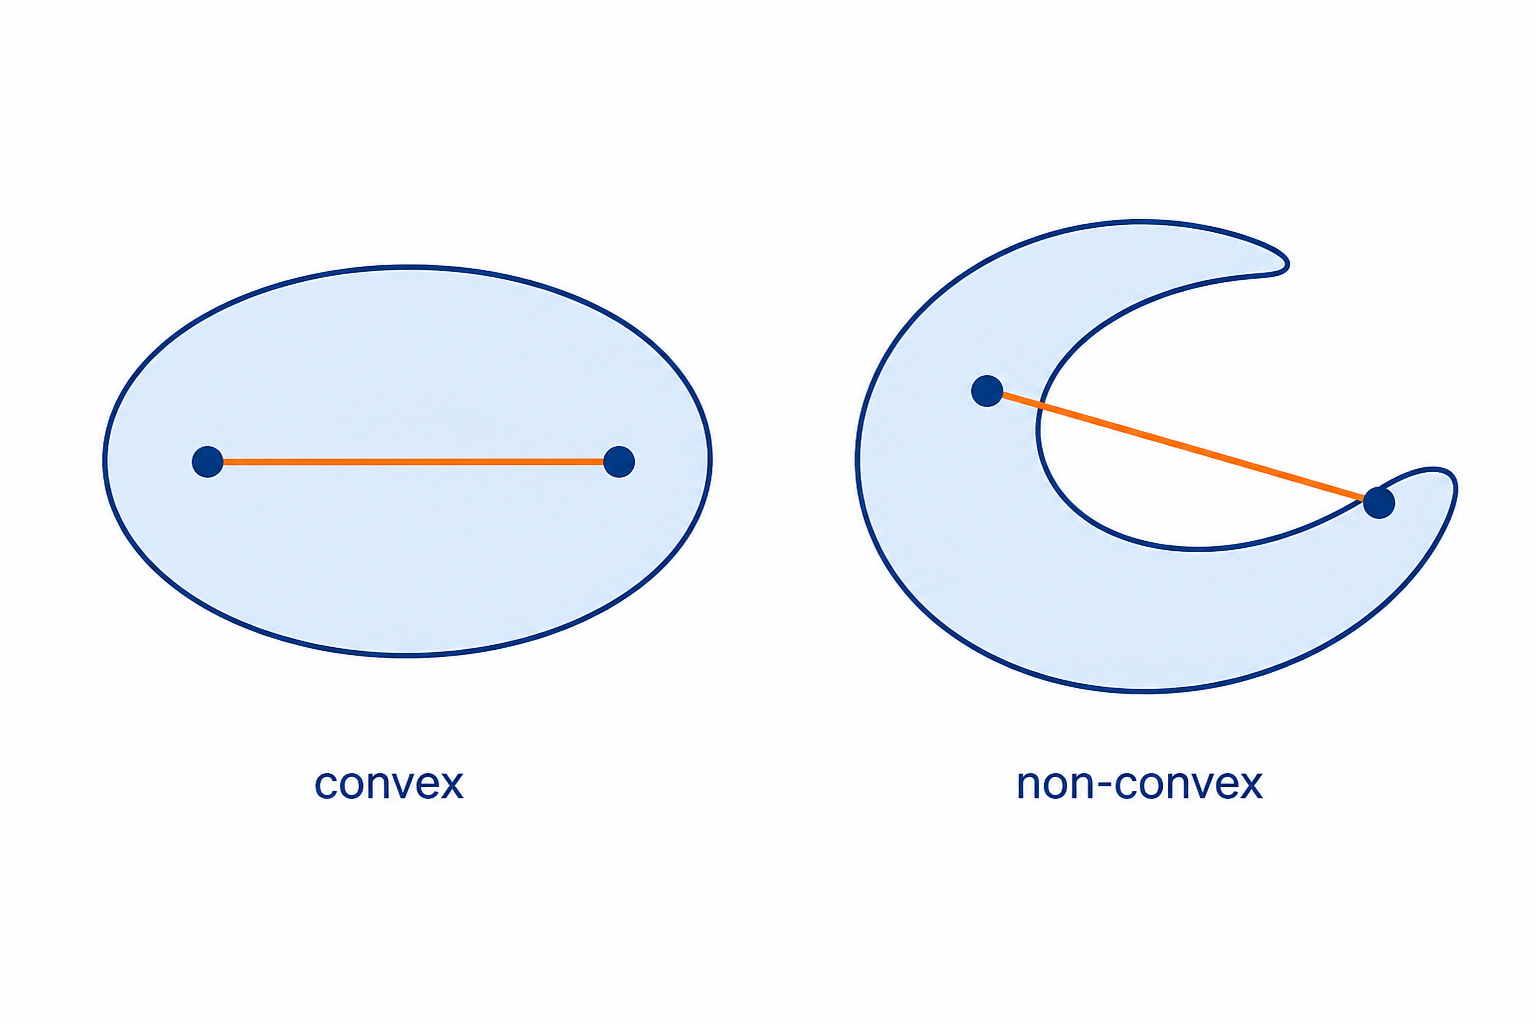
\includegraphics[width=\linewidth]{assets/convexity-set-diagram.png}
  \end{column}
  \end{columns}
\end{frame}

\begin{frame}{First-order characterization}
  \begin{resultblock}{Result -- First-order characterization of convexity}
  If $f$ is differentiable on a convex set, then
  \[
    f\text{ convex}
    \quad\Longleftrightarrow\quad
    f(y)\geq f(x)+\grad f(x)\trans(y-x)
  \]
  for all $x,y$.
  \end{resultblock}

  \begin{resultblock}{Global optimality consequence}
    If $\grad f(x^\star)=0$, then
    \[
      f(y)\geq f(x^\star)
      \qquad\forall y.
    \]
    Every stationary point of a convex function is a global minimizer.
  \end{resultblock}
\end{frame}

\begin{frame}{Second-order characterization}
  \begin{resultblock}{Result -- Hessian characterization of convexity}
  If $f$ is twice differentiable on an open convex set,
  \[
    f\text{ convex}
    \quad\Longleftrightarrow\quad
    \grad^2f(x)\succeq0
    \quad\forall x.
  \]
  \end{resultblock}

  \begin{itemize}
    \item $x\mapsto \frac12x\trans Qx+c\trans x$ is convex iff $Q\succeq0$.
    \item A nonnegative weighted sum of convex functions is convex.
    \item The pointwise maximum of convex functions is convex.
  \end{itemize}
\end{frame}

\begin{frame}{Worked Example: Prove Convexity Quickly}
  Let $x,a\in\R^d$, with $a$ fixed. Determine whether the following functions
  are convex on their natural domains:
  \[
    f(x)=e^{a\trans x},
    \qquad
    g(x)=\log(1+e^x),
    \qquad
    h(x,y)=x^2-xy+y^2.
  \]

  \pause
  \[
    \grad f(x)=e^{a\trans x}a,
    \qquad
    \grad^2f(x)=e^{a\trans x}aa\trans\succeq0,
    \qquad
    g''(x)=\frac{e^x}{(1+e^x)^2}>0.
  \]

  Indeed, for every $z\in\R^d$,
  $z\trans\grad^2f(x)z=e^{a\trans x}(a\trans z)^2\geq0$.

  \pause
  \[
    \grad^2h=\begin{pmatrix}2&-1\\-1&2\end{pmatrix}
  \]
  has eigenvalues $1$ and $3$. All three functions are convex.
\end{frame}

\begin{frame}{Your Turn: Convex or Not?}
  Determine whether the following functions are convex on $\R^2$:
  \[
    p(x,y)=x^4+e^y,
    \qquad
    q(x,y)=x^2-y^2.
  \]

  \begin{exampleblock}{Task}
    Use the Hessian criterion and justify the conclusion globally.
  \end{exampleblock}

  \pause
  \[
    \grad^2p(x,y)=\begin{pmatrix}12x^2&0\\0&e^y\end{pmatrix}\succeq0,
  \]
  hence $p$ is convex. In contrast,
  \[
    \grad^2q=\begin{pmatrix}2&0\\0&-2\end{pmatrix}
  \]
  is indefinite, so $q$ is not convex.
\end{frame}

\begin{frame}{Strong convexity and smoothness}
  $f$ is $\mu$-strongly convex if
  \[
    \grad^2f(x)\succeq \mu I.
  \]
  Its gradient is $L$-Lipschitz if
  \[
    \|\grad f(x)-\grad f(y)\|\leq L\|x-y\|,
  \]
  equivalently, for a twice differentiable $f$,
  \[
    \grad^2f(x)\preceq LI.
  \]

  The ratio
  \[
    \kappa=\frac{L}{\mu}
  \]
  measures conditioning: large $\kappa$ generally means slow first-order optimization.
\end{frame}

\begin{frame}{Worked Example: Conditioning of a Quadratic}
  Let
  \[
    f(x,y)=\frac12(x^2+100y^2).
  \]
  \textbf{Task.} Find $\mu$, $L$, and $\kappa$.

  \pause
  \[
    \grad^2f=\begin{pmatrix}1&0\\0&100\end{pmatrix}.
  \]

  \pause
  Thus
  \[
    \mu=1,
    \qquad L=100,
    \qquad \kappa=100.
  \]
  The level sets are elongated: one step size must handle two very different curvatures.
\end{frame}

\begin{frame}{Your Turn: Read Conditioning from the Hessian}
  Let
  \[
    g(x,y)=2x^2+32y^2.
  \]
  \begin{exampleblock}{Task}
    Find the strong-convexity constant $\mu$, smoothness constant $L$, and
    condition number $\kappa=L/\mu$.
  \end{exampleblock}

  \pause
  \[
    \grad^2g=\begin{pmatrix}4&0\\0&64\end{pmatrix}.
  \]
  Therefore
  \[
    \boxed{\mu=4,\qquad L=64,\qquad \kappa=16.}
  \]
  The slow direction is the $x$-axis and the steep direction is the $y$-axis.
\end{frame}

% -----------------------------------------------------------------------------
\section{Algorithms for smooth optimization}

\begin{frame}{Gradient descent}
  \begin{columns}[c,onlytextwidth]
  \begin{column}{0.53\textwidth}
  The gradient points in the direction of steepest local increase. Therefore
  \[
    \boxed{x_{k+1}=x_k-\alpha_k\grad f(x_k)}
  \]
  moves in a descent direction.

  A practical implementation needs:
  \begin{itemize}
    \item an initial point $x_0$;
    \item a step-size rule $\alpha_k$;
    \item a stopping criterion, e.g. $\|\grad f(x_k)\|\leq\varepsilon$;
    \item an iteration limit and numerical safeguards.
  \end{itemize}
  \end{column}
  \begin{column}{0.44\textwidth}
    \centering
    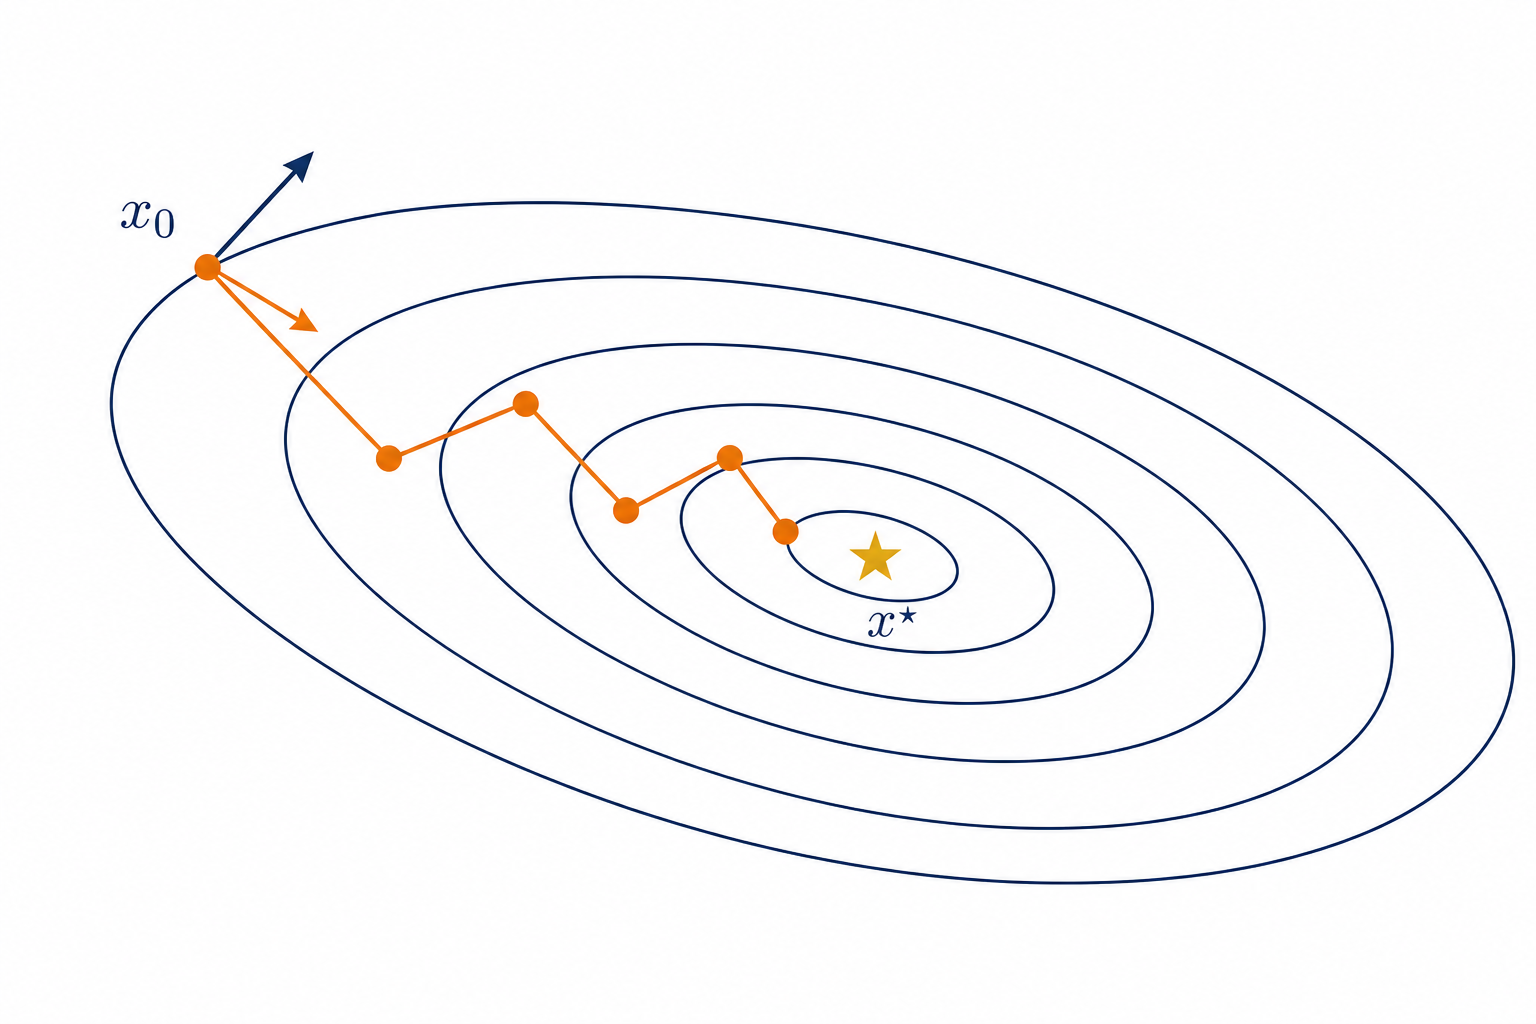
\includegraphics[width=\linewidth]{assets/gradient-descent-diagram.png}
  \end{column}
  \end{columns}
\end{frame}

\begin{frame}{How small should the step be?}
  \begin{resultblock}{Result -- Descent lemma and admissible step size}
  If $\grad f$ is $L$-Lipschitz, then
  \[
    f(x-\alpha\grad f(x))
    \leq f(x)-\alpha\left(1-\frac{L\alpha}{2}\right)\|\grad f(x)\|^2.
  \]

  Therefore every fixed step
  \[
  0<\alpha<\frac{2}{L}
  \]
  guarantees descent away from stationary points.
  \end{resultblock}

  A standard conservative choice is $\alpha=1/L$. If $L$ is unknown, use
  backtracking line search.
\end{frame}

\begin{frame}{Convergence under strong convexity}
  \begin{resultblock}{Result -- Linear convergence rate}
  If $f$ is $\mu$-strongly convex and $L$-smooth, gradient descent with
  $\alpha=1/L$ satisfies
  \[
    f(x_k)-f(x^\star)
    \leq
    \left(1-\frac{\mu}{L}\right)^k
    \bigl(f(x_0)-f(x^\star)\bigr).
  \]
  \end{resultblock}

  \begin{block}{Interpretation}
    \begin{itemize}
      \item The error decreases geometrically.
      \item A large condition number $\kappa=L/\mu$ slows convergence.
      \item Rescaling or preconditioning can change the geometry dramatically.
    \end{itemize}
  \end{block}
\end{frame}

\begin{frame}{Newton's method}
  Replace $f$ locally by its quadratic approximation:
  \[
    f(x+p)\approx f(x)+\grad f(x)\trans p+\frac12p\trans\grad^2f(x)p.
  \]
  Minimizing this model gives
  \[
    \grad^2f(x_k)p_k=-\grad f(x_k),
    \qquad
    x_{k+1}=x_k+p_k.
  \]

  \begin{alertblock}{Implementation rule}
    Solve the linear system; do not explicitly invert the Hessian.
  \end{alertblock}
\end{frame}

\begin{frame}{Gradient descent or Newton?}
  \begin{center}
    \begin{tabular}{lll}
      \toprule
      & Gradient descent & Newton \\
      \midrule
      Information & gradient & gradient + Hessian \\
      Per iteration & relatively cheap & linear solve \\
      Scaling & good for large $d$ & demanding for large $d$ \\
      Local speed & linear & often quadratic \\
      Robustness & step-size issue & Hessian may be indefinite \\
      \bottomrule
    \end{tabular}
  \end{center}

  In practice: damping, line search, quasi-Newton methods, and automatic differentiation
  bridge the gap.
\end{frame}

\begin{frame}{Projected gradient descent}
  \small
  \begin{resultblock}{Convex constrained problem and projection}
  We now want to solve the constrained convex problem
  \[
    \boxed{\min_{x\in C} f(x),}
  \]
  where $f$ is differentiable and convex, and $C$ is a nonempty closed convex set.

  The Euclidean projection onto $C$ is
  \[
    \boxed{\proj_C(z)=\argmin_{u\in C}\|u-z\|_2.}
  \]
  \end{resultblock}
  The projected-gradient update is
  \[
    x_{k+1}=\proj_C\bigl(x_k-\alpha_k\grad f(x_k)\bigr).
  \]

  Each iteration takes an unconstrained gradient step, then projects the result
  back onto the convex feasible set $C$.
\end{frame}

% -----------------------------------------------------------------------------
\section{Equality constraints and Lagrange multipliers}

\begin{frame}{Geometry of an equality constraint}
  \begin{columns}[c,onlytextwidth]
  \begin{column}{0.52\textwidth}
  Consider
  \[
    \min_x f(x)
    \quad\text{s.t.}\quad h(x)=0.
  \]
  At a regular feasible point, admissible first-order directions $v$ satisfy
  \[
    \grad h(x)\trans v=0.
  \]

  At a constrained optimum, $\grad f(x^\star)$ must also be orthogonal to every
  feasible direction. Therefore
  \[
    \grad f(x^\star)+\lambda^\star\grad h(x^\star)=0.
  \]
  \end{column}
  \begin{column}{0.45\textwidth}
    \centering
    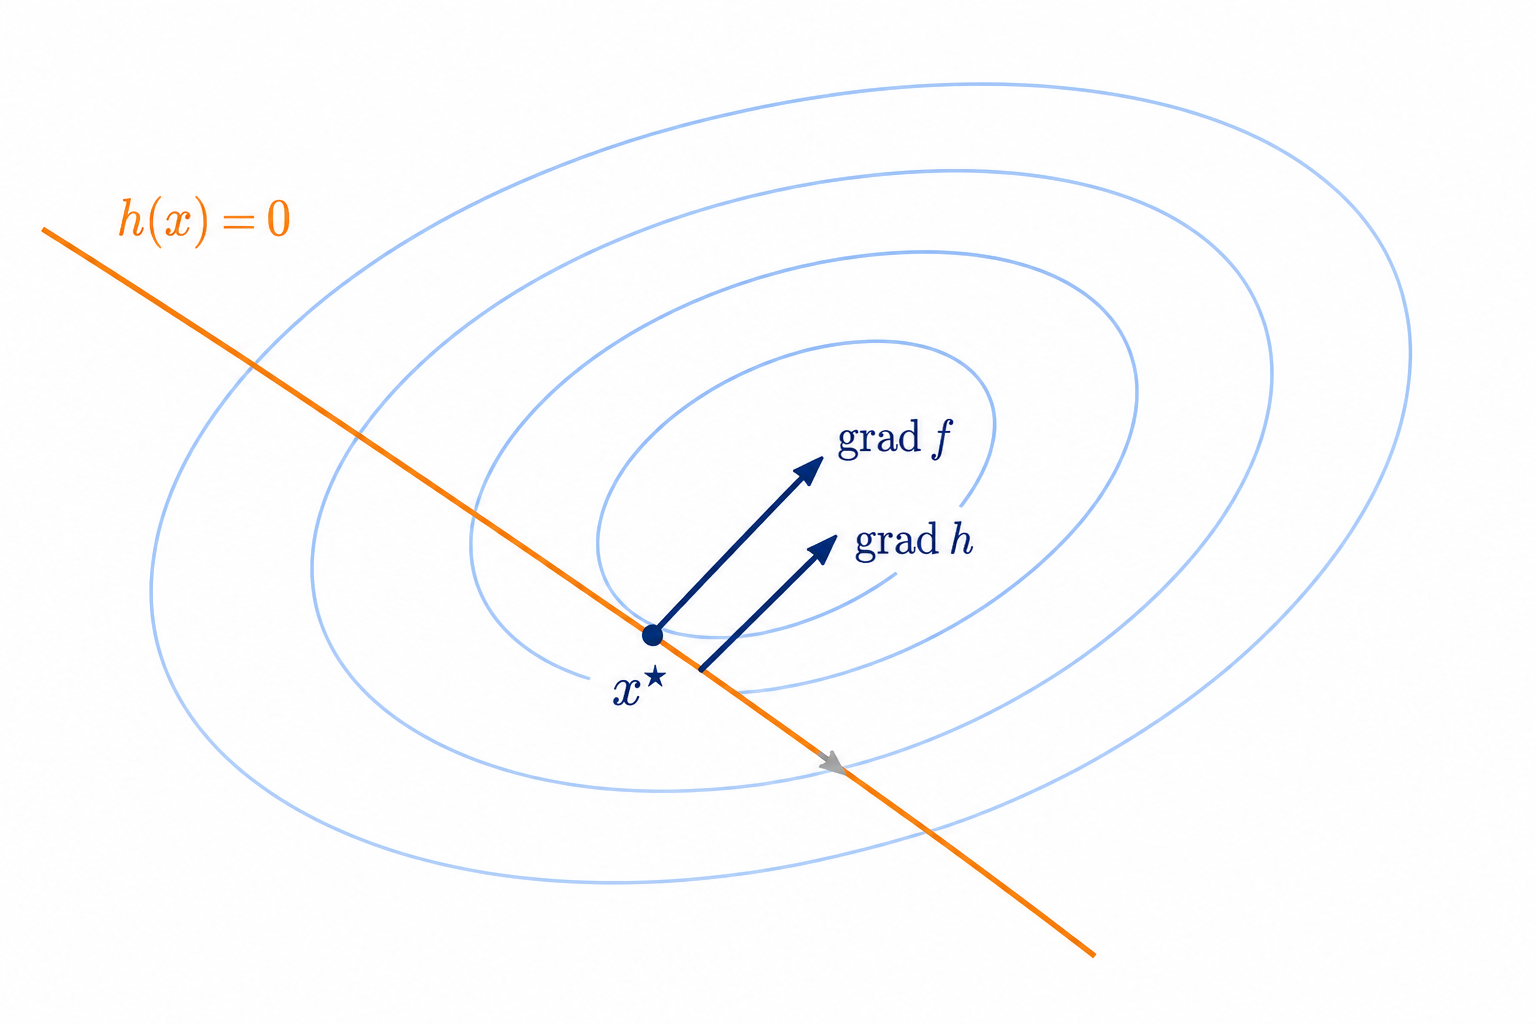
\includegraphics[width=\linewidth]{assets/lagrange-geometry-diagram.png}
  \end{column}
  \end{columns}
\end{frame}

\begin{frame}{The Lagrangian system}
  \begin{resultblock}{Result -- Lagrange first-order conditions}
  Define
  \[
    \mathcal L(x,\lambda)=f(x)+\lambda\trans h(x).
  \]
  Under a regularity condition, a constrained local optimum satisfies
  \[
    \boxed{
    \begin{aligned}
      \grad_x\mathcal L(x^\star,\lambda^\star)&=0,\\
      h(x^\star)&=0.
    \end{aligned}}
  \]
  \end{resultblock}

  \begin{alertblock}{Necessary, not sufficient in general}
    These equations generate candidates. Without convexity or a second-order
    argument, a candidate may be a maximum or a saddle point.
  \end{alertblock}
\end{frame}

\begin{frame}{Multipliers attach a price to infeasibility}
  Consider the equality-constrained primal problem
  \[
    p^\star=\min_x f(x)
    \quad\text{s.t.}\quad h(x)=0,
    \qquad \mathcal L(x,\lambda)=f(x)+\lambda\trans h(x).
  \]

  For a fixed multiplier $\lambda$, the Lagrangian replaces the hard constraint
  by a penalty or reward proportional to its violation:
  \[
    \lambda\trans h(x)=\sum_{i=1}^m\lambda_i h_i(x).
  \]

  \begin{itemize}
    \item $x$ is the \textbf{primal variable}: it chooses the decision;
    \item $\lambda$ is the \textbf{dual variable}: it prices constraint violations;
    \item a large $|\lambda_i|$ indicates that constraint $i$ strongly affects value.
  \end{itemize}

  \begin{block}{Sensitivity interpretation}
    Under regularity, the optimal multiplier measures the marginal change in the
    optimal value when the corresponding constraint is perturbed.
  \end{block}
\end{frame}

\begin{frame}{The dual function gives one bound per multiplier}
  For a fixed $\lambda$, minimize the Lagrangian over all primal decisions:
  \[
    \boxed{q(\lambda)=\inf_x \mathcal L(x,\lambda).}
  \]
  The function $q$ is concave in $\lambda$, even when the primal problem is not
  convex, because it is a pointwise infimum of affine functions of $\lambda$.

  If $x$ is feasible, then $h(x)=0$, so
  \[
    q(\lambda)
    \leq \mathcal L(x,\lambda)
    =f(x).
  \]

  \begin{block}{From a family of bounds to the dual problem}
    \[
      \boxed{d^\star=\sup_\lambda q(\lambda).}
    \]
    Each $\lambda$ produces a lower bound; the dual chooses the tightest one.
  \end{block}
\end{frame}

\begin{frame}{Weak duality leaves a measurable gap}
  \small
  Taking the best dual bound and the best feasible primal value gives
  \begin{resultblock}{Result -- Weak duality}
  \[
    \boxed{
      \underbrace{d^\star}_{\sup_\lambda q(\lambda)}
      \leq
      \underbrace{p^\star}_{\inf_{h(x)=0}f(x)}.}
  \]
  This is \textbf{weak duality}; it does not require convexity.
  \end{resultblock}

  For any primal-feasible $x$ and any multiplier $\lambda$,
  \[
    \underbrace{f(x)-q(\lambda)}_{\text{primal--dual gap}}\geq0.
  \]

  \begin{block}{Why the gap is useful}
    A small gap certifies that the primal candidate and the dual bound are close
    to optimal. Algorithms often monitor this gap as a stopping criterion.
  \end{block}
\end{frame}

\begin{frame}{Strong duality means that the best bound is exact}
  \footnotesize
  \begin{resultblock}{Result -- Strong duality}
  Strong duality means that the primal--dual gap vanishes at the optimum:
  \[
    \boxed{d^\star=p^\star.}
  \]
  \end{resultblock}
  A standard convex setting is:
  \begin{itemize}
    \item $f$ and the inequality functions are convex;
    \item equality constraints are affine;
    \item a constraint qualification holds, commonly Slater's condition.
  \end{itemize}

  \begin{alertblock}{Convexity alone is not the whole story}
    Without an appropriate regularity condition, a positive duality gap may
    remain or the dual optimum may fail to be attained.
  \end{alertblock}

  Under strong duality, solving the dual problem can recover the primal value,
  certify optimality, and sometimes be computationally easier.
\end{frame}

\begin{frame}{Strong duality turns optimization into a saddle problem}
  The primal formulation minimizes after enforcing feasibility:
  \[
    p^\star=\min_x\max_\lambda \mathcal L(x,\lambda).
  \]
  The dual formulation maximizes the best lower bound:
  \[
    d^\star=\max_\lambda\min_x \mathcal L(x,\lambda).
  \]

  When strong duality holds and optimal solutions exist,
  \[
    \boxed{
      \min_x\max_\lambda \mathcal L(x,\lambda)
      =\max_\lambda\min_x \mathcal L(x,\lambda).}
  \]
  The primal--dual solution $(x^\star,\lambda^\star)$ is a saddle point:
  \[
    \mathcal L(x^\star,\lambda)
    \leq \mathcal L(x^\star,\lambda^\star)
    \leq \mathcal L(x,\lambda^\star).
  \]

  Moving in $x$ can only increase the Lagrangian away from the minimizer, while
  moving in $\lambda$ can only decrease it away from the maximizer.
\end{frame}

\begin{frame}{Gradient descent--ascent is a primal--dual algorithm}
  For a differentiable Lagrangian, a direct saddle-point iteration is
  \[
    \boxed{
    \begin{aligned}
      x_{k+1}&=x_k-\alpha_k\grad_x\mathcal L(x_k,\lambda_k),
      &&\text{gradient descent in }x,\\
      \lambda_{k+1}&=\lambda_k+\beta_k\grad_\lambda
        \mathcal L(x_k,\lambda_k),
      &&\text{gradient ascent in }\lambda.
    \end{aligned}}
  \]
  Since $\grad_\lambda\mathcal L(x,\lambda)=h(x)$,
  \[
    \lambda_{k+1}=\lambda_k+\beta_k h(x_k).
  \]

  \begin{itemize}
    \item the primal step reduces the objective for the current multiplier;
    \item the dual step increases the price of violated constraints;
    \item step sizes and convex--concave structure determine convergence.
  \end{itemize}

  \begin{alertblock}{Practical warning}
    Simultaneous descent--ascent can oscillate. Damping, extragradient methods,
    or an augmented Lagrangian often improve stability.
  \end{alertblock}
\end{frame}

\begin{frame}{Worked Example: Minimum Distance to a Line}
  \begin{columns}[c,onlytextwidth]
  \begin{column}{0.56\textwidth}
  Solve
  \[
    \min_{x,y} x^2+y^2
    \quad\text{s.t.}\quad x+y=1.
  \]

  \pause
  \[
    \mathcal L(x,y,\lambda)=x^2+y^2+\lambda(x+y-1).
  \]
  The first-order conditions are
  \[
    2x+\lambda=0,
    \qquad 2y+\lambda=0,
    \qquad x+y=1.
  \]

  \pause
  Thus $x=y$ and
  \[
    \boxed{x^\star=y^\star=\frac12,
    \qquad \lambda^\star=-1.}
  \]
  \end{column}
  \begin{column}{0.41\textwidth}
    \centering
    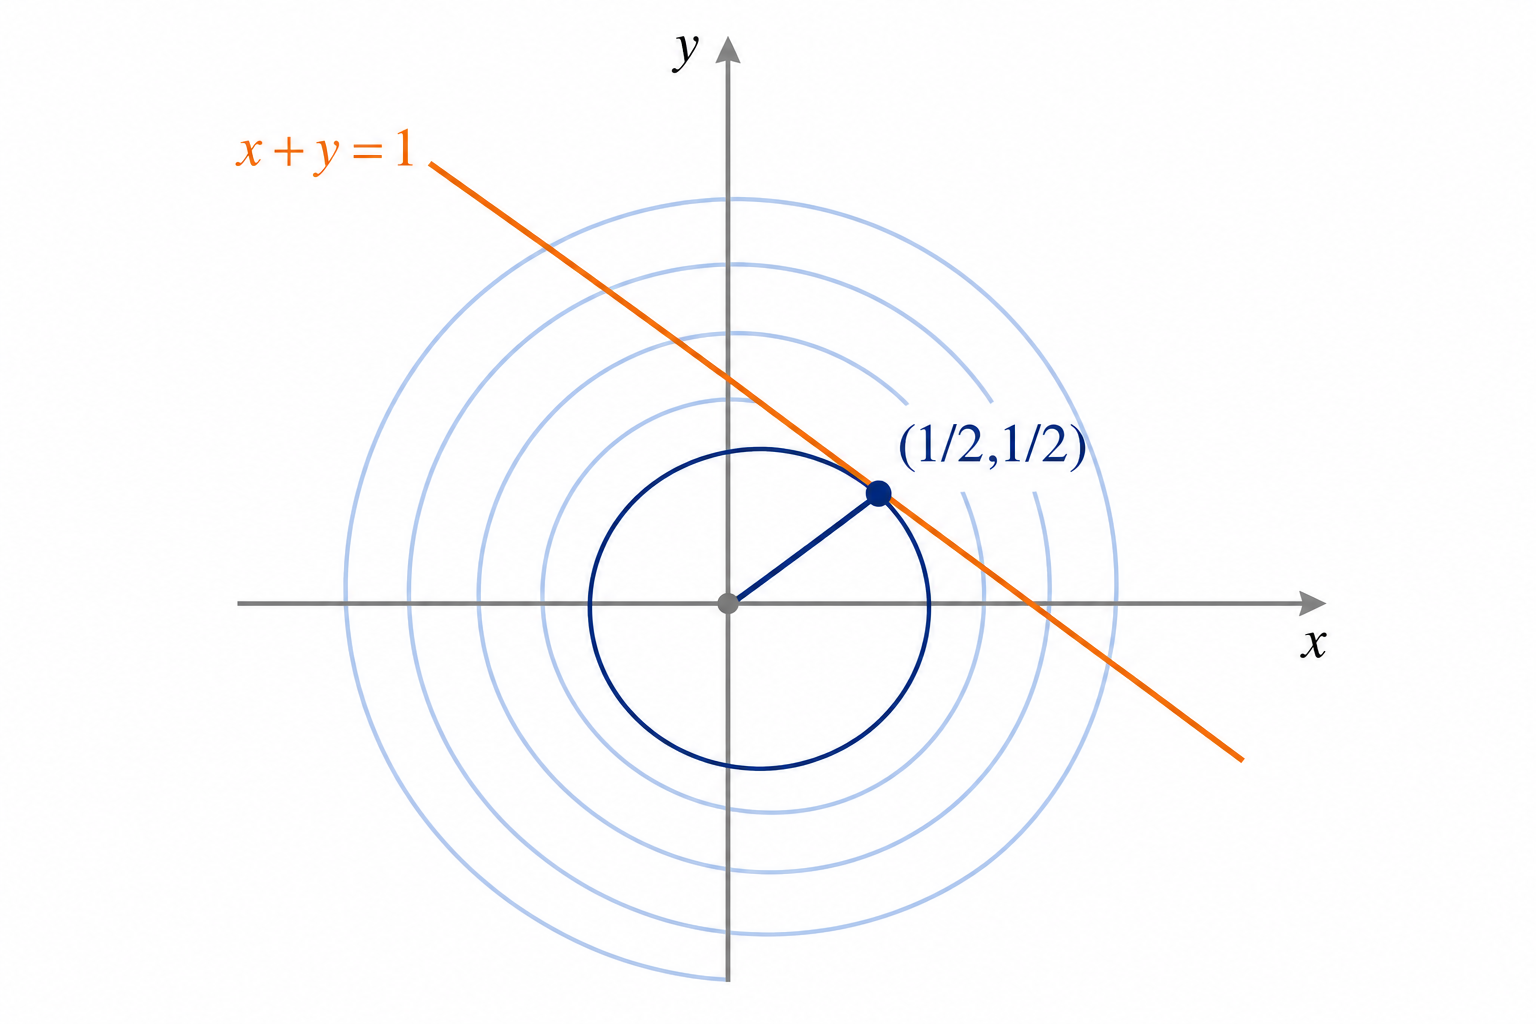
\includegraphics[width=\linewidth]{assets/min-distance-line-diagram.png}
  \end{column}
  \end{columns}
\end{frame}

\begin{frame}{Your Turn: Minimum Distance to Another Line}
  Solve
  \[
    \min_{x,y}x^2+y^2
    \quad\text{s.t.}\quad 2x-y=3.
  \]

  \begin{exampleblock}{Task}
    Write the Lagrangian and solve the three first-order equations.
  \end{exampleblock}

  \pause
  \[
    \mathcal L=x^2+y^2+\lambda(2x-y-3),
  \]
  so $2x+2\lambda=0$, $2y-\lambda=0$, and $2x-y=3$.
  Therefore
  \[
    \boxed{\lambda^\star=-\frac65,
    \qquad (x^\star,y^\star)=\left(\frac65,-\frac35\right).}
  \]
\end{frame}

\begin{frame}{Several equality constraints}
  For $h:\R^d\to\R^m$,
  \[
    \mathcal L(x,\lambda)=f(x)+\lambda\trans h(x).
  \]
  The stationarity condition is
  \[
    \grad f(x^\star)+Dh(x^\star)\trans\lambda^\star=0.
  \]

  \begin{alertblock}{LICQ: the condition to check}
    \[
      \boxed{\grad h_1(x^\star),\ldots,\grad h_m(x^\star)
      \text{ are linearly independent}.}
    \]
  \end{alertblock}
  Without regularity, Lagrange multipliers may fail to describe an optimum.
\end{frame}

\begin{frame}{Worked Example: Why Regularity Matters}
  Consider
  \[
    \min_x x
    \quad\text{s.t.}\quad x^2=0.
  \]
  The only feasible point is $x^\star=0$, so it is the optimizer.

  \textbf{Task.} Can the Lagrange stationarity equation hold?

  \pause
  \[
    \mathcal L(x,\lambda)=x+\lambda x^2,
    \qquad
    \partial_x\mathcal L(0,\lambda)=1.
  \]

  \pause
  No multiplier can make the derivative vanish. Here $h'(0)=0$, so the constraint
  gradient is not regular.
\end{frame}

\begin{frame}{Your Turn: Detect Another Failure of Regularity}
  Consider
  \[
    \min_{x,y}x+y
    \quad\text{s.t.}\quad x^2+y^2=0.
  \]
  \begin{exampleblock}{Task}
    Identify the optimizer and test the Lagrange stationarity equation.
  \end{exampleblock}

  \pause
  The feasible set contains only $(0,0)$, so it is the optimizer. However,
  \[
    \grad f(0,0)=\binom11,
    \qquad
    \grad h(0,0)=\binom00.
  \]
  No $\lambda$ can satisfy $\grad f+\lambda\grad h=0$. The constraint
  gradient vanishes, so the regularity condition fails.
\end{frame}

\begin{frame}{Application: fully invested minimum variance}
  Solve
  \[
    \min_w \frac12w\trans\Sigma w
    \quad\text{s.t.}\quad \mathbf1\trans w=1,
  \]
  Here $\Sigma\succ0$ and $\mathbf1=(1,\ldots,1)\trans\in\R^d$ is the
  \textbf{vector of ones}.

  \textbf{Task.} Derive the optimal weights.

  \pause
  \[
    \Sigma w+\lambda\mathbf1=0
    \quad\Longrightarrow\quad
    w=-\lambda\Sigma^{-1}\mathbf1.
  \]
  Enforcing the budget constraint gives
  \[
    -\lambda=\frac{1}{\mathbf1\trans\Sigma^{-1}\mathbf1}.
  \]

  \pause
  \[
    \boxed{w^\star=
    \frac{\Sigma^{-1}\mathbf1}
    {\mathbf1\trans\Sigma^{-1}\mathbf1}.}
  \]
\end{frame}

% -----------------------------------------------------------------------------
\section{Inequality constraints and KKT conditions}

\begin{frame}{KKT conditions}
  \small
  Consider
  \[
    \min_x f(x)
    \quad\text{s.t.}\quad h(x)=0,\quad g(x)\leq0,
  \]
  with
  \[
    \mathcal L(x,\nu,\lambda)=f(x)+\nu\trans h(x)+\lambda\trans g(x).
  \]
  With the convention $g(x)\leq0$, the inequality multiplier must satisfy
  $\boxed{\lambda\geq0}$; the equality multiplier $\nu$ is unrestricted.
  \begin{resultblock}{Result -- KKT necessary conditions}
  Under suitable regularity, a local optimum satisfies:
  \[
    \boxed{
    \begin{aligned}
      \grad_x\mathcal L(x^\star,\nu^\star,\lambda^\star)&=0
        &&\text{stationarity},\\
      h(x^\star)=0,\quad g(x^\star)&\leq0
        &&\text{primal feasibility},\\
      \lambda^\star&\geq0
        &&\text{dual feasibility},\\
      \lambda_i^\star g_i(x^\star)&=0
        &&\text{complementary slackness}.
    \end{aligned}}
  \]
  \end{resultblock}
\end{frame}

\begin{frame}{Active or inactive?}
  For one inequality $g(x)\leq0$:
  \begin{itemize}
    \item if $g(x^\star)<0$, the constraint is inactive and
      $\lambda^\star=0$;
    \item if $\lambda^\star>0$, complementary slackness forces
      $g(x^\star)=0$;
    \item an active constraint can still have $\lambda^\star=0$.
  \end{itemize}

  \begin{block}{Practical method}
    Guess the active set, solve the corresponding equations, then verify all signs
    and inequalities.
  \end{block}
\end{frame}

\begin{frame}{Hands-on: an inactive constraint}
  Solve
  \[
    \min_x (x-2)^2
    \quad\text{s.t.}\quad x\geq1.
  \]
  Write $g(x)=1-x\leq0$.

  \pause
  \[
    \mathcal L(x,\lambda)=(x-2)^2+\lambda(1-x),
  \]
  and stationarity gives
  \[
    2(x-2)-\lambda=0.
  \]

  \pause
  The unconstrained minimizer $x^\star=2$ is feasible and strictly inside the set.
  Hence
  \[
    \boxed{x^\star=2,
    \qquad \lambda^\star=0.}
  \]
\end{frame}

\begin{frame}{Hands-on: a binding constraint}
  Solve
  \[
    \min_x x^2
    \quad\text{s.t.}\quad x\geq1.
  \]

  \pause
  With $g(x)=1-x\leq0$,
  \[
    \mathcal L(x,\lambda)=x^2+\lambda(1-x),
    \qquad
    2x-\lambda=0.
  \]

  \pause
  The constraint must bind, so $x^\star=1$. Stationarity then gives
  \[
    \boxed{x^\star=1,
    \qquad \lambda^\star=2.}
  \]
  All four KKT conditions are satisfied.
\end{frame}

\begin{frame}{Worked Example: A Two-Dimensional Boundary}
  Solve
  \[
    \min_{x,y}(x-1)^2+(y-2)^2
    \quad\text{s.t.}\quad x+y\leq1.
  \]

  \pause
  With $g(x,y)=x+y-1$,
  \[
    2(x-1)+\lambda=0,
    \qquad
    2(y-2)+\lambda=0.
  \]
  Hence $x=1-\lambda/2$ and $y=2-\lambda/2$.

  \pause
  The unconstrained point $(1,2)$ is infeasible, so the constraint binds:
  \[
    x+y=3-\lambda=1.
  \]
  Thus
  \[
    \boxed{\lambda^\star=2,
    \qquad (x^\star,y^\star)=(0,1).}
  \]
\end{frame}

\begin{frame}{Your Turn: Project onto a Half-Space}
  Solve
  \[
    \min_{x,y}(x-2)^2+(y+1)^2
    \quad\text{s.t.}\quad x-y\leq1.
  \]

  \begin{exampleblock}{Task}
    Determine whether the constraint binds, then solve the KKT equations.
  \end{exampleblock}

  \pause
  The unconstrained point $(2,-1)$ violates $x-y\leq1$. With
  $g(x,y)=x-y-1$,
  \[
    x=2-\frac\lambda2,
    \qquad y=-1+\frac\lambda2.
  \]
  Binding feasibility gives $3-\lambda=1$, hence
  \[
    \boxed{\lambda^\star=2,
    \qquad (x^\star,y^\star)=(1,0).}
  \]
\end{frame}

\begin{frame}{When KKT is sufficient}
  \begin{resultblock}{Result -- Convex KKT sufficiency}
  Suppose:
  \begin{itemize}
    \item $f$ and every $g_i$ are convex;
    \item every equality constraint is affine;
    \item a constraint qualification holds.
  \end{itemize}

  Then any point satisfying the KKT conditions is a \textbf{global optimum}.
  \end{resultblock}

  \begin{alertblock}{Nonconvex problems}
    KKT conditions are generally only necessary local conditions. Candidate points
    still need to be compared or classified.
  \end{alertblock}
\end{frame}

% -----------------------------------------------------------------------------
\section{Portfolio optimization}

\begin{frame}{Returns and risk become an optimization problem}
  For $d$ assets, let $R=(R_1,\ldots,R_d)\trans\in\R^d$ be the
  \textbf{random vector of asset returns} over one investment period, and let
  \[
    w\in\R^d,
    \qquad \mu=\E[R],
    \qquad \Sigma=\operatorname{Cov}(R).
  \]
  Then
  \[
    \E[w\trans R]=\mu\trans w,
    \qquad
    \operatorname{Var}(w\trans R)=w\trans\Sigma w.
  \]

  Typical portfolio constraints are
  \[
    \mathbf1\trans w=1,
    \qquad w\geq0,
    \qquad \ell\leq w\leq u.
  \]
  When $\Sigma\succeq0$, variance is a convex quadratic objective.
\end{frame}

\begin{frame}{Mean--variance optimization balances two objectives}
  A standard formulation is
  \[
    \boxed{
    \min_w\ \frac12w\trans\Sigma w-\gamma\mu\trans w
    \quad\text{s.t.}\quad \mathbf1\trans w=1.}
  \]
  Here $\gamma>0$ controls the reward assigned to expected return.

  \begin{exampleblock}{Derive the first-order system}
    Write the Lagrangian and solve for $w$ in terms of the multiplier.
  \end{exampleblock}

  \pause
  \[
    \Sigma w-\gamma\mu+\lambda\mathbf1=0,
    \qquad \mathbf1\trans w=1.
  \]
  Thus
  \[
    w=\Sigma^{-1}(\gamma\mu-\lambda\mathbf1),
  \]
  with $\lambda$ determined by the budget constraint.
\end{frame}

\begin{frame}{A target return traces the efficient frontier}
  Fix a target return $m$. The minimum-risk portfolio solves
  \[
    \min_w\frac12w\trans\Sigma w
    \quad\text{s.t.}\quad
    \mathbf1\trans w=1,
    \quad \mu\trans w=m.
  \]
  Define
  \[
    C=\begin{pmatrix}\mathbf1\trans\\\mu\trans\end{pmatrix},
    \qquad d=\begin{pmatrix}1\\m\end{pmatrix}.
  \]

  \pause
  The equality-constrained quadratic formula gives
  \[
    \boxed{w^\star=\Sigma^{-1}C\trans
    (C\Sigma^{-1}C\trans)^{-1}d.}
  \]
  Varying $m$ generates the efficient frontier in mean--variance space.
\end{frame}

\begin{frame}{Long-only portfolios use KKT conditions}
  Add the constraints $w_i\geq0$, written as $-w_i\leq0$:
  \[
    \min_w\frac12w\trans\Sigma w-\gamma\mu\trans w
    \quad\text{s.t.}\quad
    \mathbf1\trans w=1,
    \quad -w\leq0.
  \]
  The KKT stationarity equation is
  \[
    \Sigma w-\gamma\mu+\lambda\mathbf1-\eta=0,
  \]
  with
  \[
    w\geq0,
    \qquad \eta\geq0,
    \qquad \eta_iw_i=0.
  \]

  Since the problem is convex, KKT conditions are sufficient under the usual
  constraint qualification.
\end{frame}

\begin{frame}{Real portfolios add operational constraints}
  Practical models commonly include
  \begin{itemize}
    \item position bounds $\ell_i\leq w_i\leq u_i$;
    \item sector or factor-exposure limits;
    \item turnover control $\|w-w^{\mathrm{old}}\|_1\leq\tau$;
    \item transaction costs and tracking error;
    \item stress constraints across several scenarios.
  \end{itemize}

  \begin{block}{Modeling principle}
    Preserve convexity when possible: quadratic risk with linear constraints is
    a quadratic program that can be solved reliably at realistic scale.
  \end{block}
\end{frame}

\begin{frame}{Hands-on synthesis: constrained rebalancing}
  \small
  Consider
  \[
    \min_w
    \frac12w\trans\Sigma w-\gamma\mu\trans w
  \]
  subject to
  \[
    \mathbf1\trans w=1,
    \qquad w\geq0,
    \qquad \|w-w^{\mathrm{old}}\|_2^2\leq\tau^2.
  \]

  \textbf{Task.} Write the KKT conditions and identify the appropriate solver.

  \pause
  Introduce $\lambda\in\R$, $\eta\geq0$ for $-w\leq0$, and $\rho\geq0$ for
  $\|w-w^{\mathrm{old}}\|_2^2-\tau^2\leq0$. Then
  \[
  \boxed{
  \Sigma w-\gamma\mu+\lambda\mathbf1-\eta
  +2\rho(w-w^{\mathrm{old}})=0.}
  \]
  Together with primal and dual feasibility, complementary slackness is
  \[
  \boxed{
  \eta_iw_i=0\quad\forall i,
  \qquad
  \rho\bigl(\|w-w^{\mathrm{old}}\|_2^2-\tau^2\bigr)=0.}
  \]
  When $\Sigma\succeq0$, this is a convex quadratically constrained quadratic
  program; under the usual qualification, KKT is sufficient and a convex
  QCQP solver returns the global optimum.
\end{frame}

% -----------------------------------------------------------------------------
\section{Putting the toolkit to work}

\begin{frame}{A robust problem-solving checklist}
  \begin{enumerate}
    \item Write the decision variable, objective, and feasible set.
    \item Check dimensions, differentiability, and convexity.
    \item Compute first-order conditions.
    \item Use Hessian information or convexity to classify candidates.
    \item For constraints, state a sign convention and write all KKT conditions.
    \item Choose an algorithm that respects the structure.
    \item Verify feasibility, stationarity, and numerical convergence.
    \item Interpret the result in the original application.
  \end{enumerate}
\end{frame}

\begin{frame}{Final challenge}
  Consider the ridge-regression problem
  \[
    \min_x \frac12\|Ax-b\|_2^2+\frac{\lambda}{2}\|x\|_2^2,
    \qquad \lambda>0.
  \]
  \textbf{Tasks.}
  \begin{enumerate}
    \item Prove that the objective is strongly convex.
    \item Derive the unique minimizer.
    \item Write one gradient-descent iteration.
  \end{enumerate}

  \pause
  \[
    \grad f(x)=A\trans(Ax-b)+\lambda x,
    \qquad
    \grad^2f(x)=A\trans A+\lambda I\succeq\lambda I.
  \]
  \pause
  \[
    \boxed{x^\star=(A\trans A+\lambda I)^{-1}A\trans b,}
    \qquad
    x_{k+1}=x_k-\alpha\bigl(A\trans(Ax_k-b)+\lambda x_k\bigr).
  \]
\end{frame}

\begin{frame}{Model choice: what structure do we see?}
  \begin{center}
    \begin{tabular}{ll}
      \toprule
      Structure & Natural first method \\
      \midrule
      smooth, unconstrained, large scale & gradient / quasi-Newton \\
      smooth, accurate local solve & Newton / damped Newton \\
      simple convex set & projected gradient \\
      equality constraints & Lagrange system \\
      convex inequalities & KKT / convex solver \\
      long-only portfolio with bounds & quadratic-programming solver \\
      quadratic objective and linear constraints & QP solver \\
      \bottomrule
    \end{tabular}
  \end{center}

  Before choosing an algorithm, identify convexity, smoothness, constraints, and
  problem dimension.
\end{frame}

\end{document}
